\section{Problem Statement}
\label{sec:problem}  
%Electricity in Colombia is predominantly generated from hydroelectric (66.8$\%$) and thermal methods (30.5$\%$), complemented by a smaller contribution from alternative means (2.7$\%$) \cite{Corficolombiana2024}. In this setup, water is essential, largely hinging on the state of rivers and reservoirs, which are presently at 72.4$\%$ of their optimal level \cite{Unigas2023Panorama}. However, the energy sector is currently facing significant hurdles. XM, the overseer of the Sistema Interconectado Nacional(SIN), has indicated congestion issues within the power network, especially in areas such as the Atlantic Coast and Chocó. The \gls*{upme} associates this with a 5$\%$ increase in electricity demand, a notable challenge for the latter part of 2023 and the beginning of 2024. Moreover, the El Niño phenomenon is a looming threat, likely to alter climatic patterns and affect hydroelectric output.

%In light of the impacts of climate change on power supply, it is imperative to consider alternative investments to enhance the reliability of the system. The push for energy diversification necessitates turning to thermal plants as a backup during emergencies. As a more environmentally friendly option due to its lower carbon dioxide emissions compared to diesel, gasoline, and coal, natural gas is gaining global prominence \cite{Unigas2023Panorama}. However, its effective utilization hinges on the complex task of transporting it via extensive pipeline networks \cite{rios2015optimization}. To achieve this efficiently, the creation of a mathematical optimization model is vital, aimed at reducing operational costs and managing flows in an effective manner\cite{wu2018operation}.

The integration of deep learning models into automatic question answering tasks, particularly in the domain of information extraction from web pages, introduces a significant challenge characterized by the inherent opacity of these models. The prevailing issue at hand is the limited interpretability inherent in current deep learning architectures, resulting in a critical obstacle to the practical efficacy and trustworthiness of such systems; due to the lack of quantitative measures that allow quantifying the relevance of each of the tokens when carrying out a task such as EQA. (\cite{yusuf2022analysis}). 

Despite notable strides in achieving high accuracy rates in response generation, the dearth of transparency hampers our ability to comprehend the rationale underpinning the model's decision-making process. This lack of interpretability not only constrains the system's utility but also impedes our capacity to optimize and refine these models for improved performance (\cite{gao2023improve}). Furthermore, improved interpretability is crucial in identifying and mitigating potential biases within the model, offering a critical means to ensure fairness and ethical deployment of artificial intelligence in question answering tasks.

\begin{figure}[h!]
    \centering%width=0.7\linewidth
    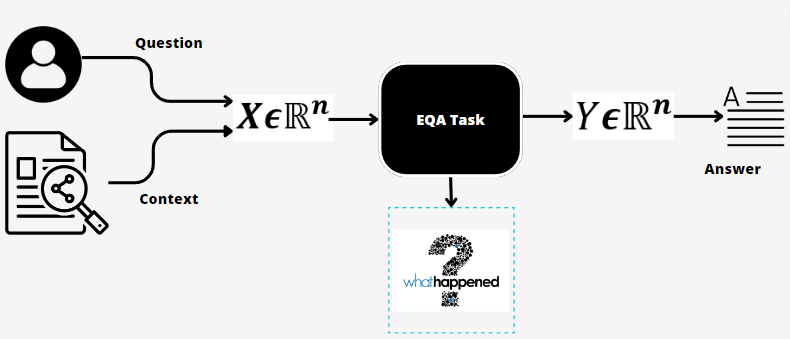
\includegraphics[width=\linewidth]{Figures/Preliminares/problem_statement.png}
    \caption{Problem Statement: Transformers have improved the state of the art in EQA task, however, the success of the transformer models has not been duly explained for this task.}
    \label{fig:problem}
\end{figure}

\newpage

\section{Research Question}
For these reasons, the central research question emerges: Can we propose a new interpretability or token-level relevance technique for question answering tasks? Or can we enhance the performance of an existing interpretability or token-level relevance technique in the state of the art, making it more robust in question answering tasks?

%======================================================================
% state of the art are related with, transfer learning, data augmentation until RFF. 

% Ir de lo más simple a los más complejo
%Addressing nonlinear optimization presents significant challenges, including convexity and convergence \textbf{[Sergei Schreider et al., 2014]}, as well as the intricate nature of iterative methods \textbf{[Minsoo et al., 2023]}. These elements are crucial to the structure of such models. Questions such as the choice of starting points, non-differentiability, and susceptibility to alterations require careful analysis \textbf{[Wei Huang et al., 2023; Muxuan Han et al., 2023]}. Additionally, the dependence on first- and second-order conditions in many traditional approaches \textbf{[Andrew Cotter et al., 2019; Guohua Gao et al., 2022]} introduces additional restrictions. Thus, challenges related to convergence, the choice of starting points, and the susceptibility to alterations in the resolution of nonlinear optimization problems will be examined.


%----------------------------------------------------------------------


%======================================================================
